\documentclass[12pt, a4paper]{article}

\usepackage[utf8x]{inputenc}
\usepackage[greek, english]{babel}
\usepackage{caption}
\usepackage[section]{placeins}
\usepackage{balance}
\usepackage{dblfloatfix}
\usepackage{hyperref}
\usepackage{color}
\usepackage{graphicx}
\usepackage{float}
\usepackage{tikz}
\usepackage{amsfonts} 

\usetikzlibrary{shapes.geometric, arrows}
\tikzstyle{stage} = [rectangle, rounded corners, minimum width=3cm, minimum height=1cm,text centered, draw=black]
\tikzstyle{arrow} = [thick,->,>=stealth]


%\usepackage[margin=2cm]{geometry}
%\usepackage{graphicx,wrapfig,lipsum}

\newcommand{\en}{\selectlanguage{english}}
\newcommand{\gr}{\selectlanguage{greek}}

\hypersetup{
	colorlinks=true,
	linkcolor=blue,
	filecolor=magenta,
	urlcolor=blue,
}

\begin{document}
	
\gr
\begin{titlepage}
	
	\begin{center}
		\vspace*{0.5cm}
		
		\LARGE
		\textbf{\normalsize ΑΝΑΓΝΩΡΙΣΗ ΔΡΑΣΤΗΡΙΟΤΗΤΑΣ ΜΕ ΧΡΗΣΗ ΑΙΣΘΗΤΗΡΩΝ ΚΙΝΗΣΗΣ}
		
		\vspace{0.5cm}
		%\LARGE
		%\Large 
		%\gr{}
		
		\vspace{1.5cm}
		
		\textbf{Γεώργιος Βαρδάκας}
		
		\vfill
		
\includegraphics[width=0.5\textwidth]{logo.png}
		
		\textbf{\normalsize Επιστημονικός υπεύθυνος έργου: \\ Στέργιος Αναστασιάδης (Αναπληρωτής Καθηγητής)}
		\vfill
		
		\textbf{\normalsize Επιβλέπων Καθηγητής: \\ Αριστείδης Λύκας (Καθηγητής)}
		
		\vspace{0.8cm}
		
		\Large
		Τμήμα Μηχανικών Η/Υ και Πληροφορικής\\
		Πολυτεχνική Σχολή Πανεπιστημίου Ιωαννίνων\\
		%Ελλάδα\\
		\date{\today}
		
	\end{center}
\end{titlepage}


\tableofcontents
\newpage

\gr
\section{Εισαγωγή}
Στην παρούσα εργασία μελετήθηκε η δυνατότητα επίλυσης του προβλήματος της {\bf αυτόματης κατάτμησης και κατηγοριοποίησης της πολυδιάστατης χρονοσειράς αισθητηριακών σημάτων} στα πλαίσια του έργου {\bf "\en HOMORE: \gr ΕΞΥΠΝΟ ΣΥΣΤΗΜΑ ΠΑΡΑΚΟΛΟΥΘΗΣΗΣ ΤΗΣ ΦΥΣΙΟΛΟΓΙΚΗΣ ΔΙΑΒΙΩΣΗΣ ΗΛΙΚΙΩΜΕΝΩΝ ΣΕ ΑΣΤΙΚΕΣ ΚΑΙ ΑΓΡΟΤΙΚΕΣ ΠΕΡΙΟΧΕΣ"} με κωδικό {\bf 82475} και Επιστημονικά Υπεύθυνο τον κ. Στέργιο Αναστασιάδη, του Επιχειρησιακού Προγράμματος Ε.Σ.Π.Α. Για τον σκοπό αυτό αρχικά συλλέχθηκαν τα δεδομένα που είναι απαραίτητα για την κατασκευή ενός μαθηματικού μοντέλου μηχανικής μάθησης, και στην συνέχεια πραγματοποιήθηκε η προ-επεξεργασία τους, ώστε να έχουν την κατάλληλη μορφή για την μετ' έπειτα εισαγωγή τους στο μοντέλο. για να εισαχθούν στο μοντέλο. Επιπρόσθετα, μελετήθηκαν διάφορα μοντέλα μηχανικής μάθησης μέχρι την εύρεση εκείνου με τα καλύτερα αποτελέσματα. Το τελικό και συνάμα βέλτιστο μοντέλο περιέχει εσωτερικά τα βήματα της προ-επεξεργασίας αλλά και της πρόβλεψης με αυτόματο τρόπο και βασίστηκε σε μεγάλο βαθμό στην μεθοδολογία \cite{arXiv:1802.01489}. Τέλος, αξίζει να σημειωθεί ότι η αξιολόγηση του μοντέλου για τον έλεγχο της ποιότητας των αποτελεσμάτων του πραγματοποιήθηκε με \en (group) K-fold cross validation\gr. Η παρούσα εργασία υπάρχει διαθέσιμη και στο παρακάτω σύνδεσμο \en \href{https://github.com/giorgosVardakas/Positional-Signal-Processing}{https://github.com/giorgosVardakas/Positional-Signal-Processing}.\gr 

\section{Συλλογή Δεδομένων}
Μία προαπαίτηση για την κατασκευή ενός μαθηματικού μοντέλου μηχανικής μάθησης είναι η ύπαρξη των απαραίτητων δεδομένων, καθώς αυτές οι μέθοδοι εκπαιδεύονται μέσω αυτών. Για την συλλογή των δεδομένων έγινε χρήση του έξυπνου ρολογιού \en Fitbit Versa\gr. Το έξυπνο αυτό ρολόι, μας δίνει την δυνατότητα να αντλήσουμε τις μετρήσεις που καταγράφουν οι διαθέσιμοι αισθητήρες του, μέσω του λογισμικού που αναπτύχθηκε στα πλαίσια του έργου \en Homore \gr από τους Θεοφάνη Μπαλάσκα και Ιορδάνη-Ραφήλ Φυδανάκη. Οι αισθητήρες αυτοί αποτελούνται από το γυροσκόπιο, το επιταχυνσιόμετρο καθώς και τον αισθητήρα καρδιακών παλμών. Οι αισθητήρες του γυροσκοπίου και του επιταχυνσιομέτρου καταγράφουν μετρήσεις με συχνότητα $10$ \en Hz \gr ενώ ο αισθητήρας καρδιακών παλμών καταγράφει μετρήσεις με συχνότητα $1$ \en Hz\gr. Στην παρούσα εργασία έγινε χρήση μόνο των αισθητήρων του γυροσκοπίου και του επιταχυνσιομέτρου καθώς οι καταγραφές του αισθητήρα των καρδιακών παλμών δεν περιείχε χρήσιμη πληροφορία για την αυτόματη κατηγοριοποίηση της πολυδιάστατης χρονοσειράς των αισθητήρων. Το τελικό σύνολο των δεδομένων που συγκεντρώθηκε και επεξεργάστηκε βασίζεται σε εφτά διαφορετικούς χρήστες. Η σχετική απεικόνιση των δεδομένων παρατίθεται στον παρακάτω πίνακα.

\begin{figure}[H]
	\centering
	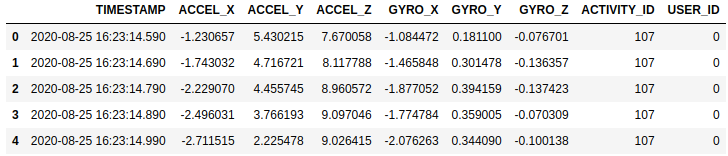
\includegraphics[width=1\textwidth, height=0.25\textheight]{Data.png}
	
	\caption{Πρώτες πέντε εγγραφές του πίνακας δεδομένων.}
	\label{fig:Data}
\end{figure}
\noindent
Πιο συγκεκριμένα, η κολόνα \en TIMESTAMP \gr αναφέρεται στο χρόνο δειγματοληψίας της εγγραφής, η κολόνα \en ACCEL\_\{X,Y,Z\} \gr στην μέτρηση του επιταχυνσιομέτρου στον άξονα \{$x, y, z$\}, η κολόνα \en GYRO\_\{X,Y,Z\} \gr στην μέτρηση του γυροσκοπίου στον άξονα \{$x, y, z$\}, η κολόνα \en ACTIVITY\_ID \gr την δραστηριότητα που πραγματοποιεί ο χρήστης και τέλος η κολόνα \en USER\_ID \gr αντιστοιχεί στο μοναδικό \en ID \gr του χρήστη που πραγματοποίησε την δραστηριότητα. Οι μετρήσεις των αισθητήρων καταγράφουν δείγματα στον τρισδιάστατο χώρο, αυτός είναι και ο λόγος που κάθε αισθητήρας έχει μετρήσεις τριών τυχαίων μεταβλητών ($x, y, z$). Με βάση αυτή την επεξεργασία και κατηγοριοποίηση τα δεδομένα έχουν κατασκευαστεί και αποθηκευτεί με τέτοιο τρόπο, ώστε να είναι έτοιμα για να χρησιμοποιηθούν για το πρόβλημα της αυτόματης ταξηνόμησης ακολουθίας $\{(X_{i}, y_{i})\}_{i=1}^{N}$, με κατηγορία $y_{i}$ για κάθε ακολουθία $X_{i}$. Η κάθε ακολουθία $X_{i}$ μοντελοποιείται σαν πολυδιάστατη χρονοσειρά αισθητηριακών σημάτων, έχοντας $Τ_{i}$ δείγματα $\left<x_{1}, x_{2}, ..., x_{T_{i}}\right>_{i}$, με κατηγορία δραστηριότητας $y_{i}$ όπου $x_{j} = [ACCEL\_X, ACCEL\_Y, ACCEL\_Z, GYRO\_X, GYRO\_Y, GYRO\_Z]_{j}$ καθώς και $y_{j} = ACTIVITY\_ID$. Αξίζει να σημειωθεί ότι για την διαχείρηση των δεδομένων έγινε χρήση της βιβλιοθήκης \en pandas \gr \cite{reback2020pandas}.

\section{Αυτόματη Kατάτμηση}
Μετά την συλλογή των δεδομένων που μοντελοποιούνται σαν πολυδιάστατη χρονοσειρά αισθητηριακών σημάτων ακολουθεί η προ-επεξεργασία τους. Το πρώτο βασικό βήμα της προ-επεξεργασίας είναι η αυτόματη κατάτμηση του σήματος. Για την επίτευξη της αυτόματης κατάτμησης έγινε χρήση της συνάρτησης \en Segment(width, overlap) \gr της βιβλιοθήκης \en seglearn \cite{arXiv:1803.08118}\gr. Η συνάρτηση λαμβάνει ως είσοδο το αρχικό σήμα και το τμηματοποιεί σε τμήματα μεγέθους \en width\gr, κάνοντας χρήση ενός επικαλυπτόμενου κυλιόμενου παραθύρου (\en sliding window\gr) σταθερού μήκος. Πιο συγκεκριμένα στην περίπτωσή μας το \en width \gr είναι ίσο με 5 δευτερόλεπτα. Με αυτήν την μέθοδο κατασκευάζουμε ένα τρισδιάστατο χρονικό τένσορα $\phi_{i} = \left<W_{1}, ..., W_{M}\right>$ για κάθε χρονοσειρά $X_{i}$. Ο τένσορας $\phi_{i}$ έχει σχήμα $\left(M_{i}, width, 6\right)$ με $width$ το μήκος του παραθύρου και $M_{i}$ τον αριθμό των παραθύρων που κατασκευάστηκαν για κάθε χρονοσειρά $X_{i}$. Το τελικό σύνολο δεδομένων είναι το σύνολο όλων των τμημάτων που παρήχθησαν από το κυλιόμενο παράθυρο και συμβολίζεται $\{W_{i}, y_{i}\}_{i=1}^{N_{w}}$, όπου το $N_{w}$ είναι το πλήθος των τμημάτων του συνόλου δεδομένων. Το πρόβλημα μηχανικής μάθησης της ταξινόμησης των πολυδιάστατων χρονοσειρών του έργου μετασχηματίστηκε, διατυπώθηκε και αξιολογήθηκε ως ταξινόμηση του τμηματοποιημένου συνόλου δεδομένων $\{W_{i}, y_{i}\}_{i=1}^{N_{w}}$.

\section{Εξαγωγή Χαρακτηριστικών}
Το επόμενο βήμα είναι η εξαγωγή των χαρακτηριστικών $F = \mathcal{F}(W)$ του τμηματοποιημένου συνόλου δεδομένων $\{W_{i}, y_{i}\}_{i=1}^{N_{w}}$. Πιο συγκεκριμένα, για κάθε τμήμα $W_{i}$ εξήχθησαν κάποια στατιστικά μεγέθη τα οποία στην συνέχεια θα αποτελέσουν την είσοδο για τον αλγόριθμο της μηχανικής μάθησης. Με αυτήν την ενέργεια από τον χώρο του τμηματοποιημένου σήματος $\{W_{i}, y_{i}\}_{i=1}^{N_{w}}$, μεταφερόμαστε στον χώρο των χαρακτηριστικών $\{F_{i}, y_{i}\}_{i=1}^{N_{w}}$. Αυτή η διαδικασία γίνεται για κάθε τυχαία μεταβλητή του τμήματος $W_{i}$ ξεχωριστά. Μερικά από τα χαρακτηριστικά (στατιστικά μεγέθη) που χρησιμοποιήθηκαν είναι η μέση τιμή, η διάμεσος, το άθροισμα των τετραγώνων, η τυπική απόκλιση, η διακύμανση, το μέγιστο και ελάχιστο στοιχείο, η λοξότητα, η κύρτωση, η μέση φασματική ενέργεια, το μέσο όρο των απόλυτων τιμών, η ρίζα των μέσων τετραγώνων κα.

\section{Προ-επεξεργασία Χαρακτηριστικών}
Στην συνέχεια ακολούθησε η κανονικοποίηση των δεδομένων εκπαίδευσης με βάση τα χαρακτηριστικά που εξαγάγαμε στο προηγούμενο βήμα. Η κανονικοποίηση του συνόλου δεδομένων είναι μια κοινή απαίτηση για πολλούς εκτιμητές μηχανικής μάθησης. Συνήθως αυτό γίνεται αφαιρώντας το μέσο όρο και κλιμακώνοντας τη διακύμανση στη μονάδα. Ωστόσο, οι υπερβολικές τιμές (\en outliers\gr) μπορούν συχνά να επηρεάσουν τη μέση τιμή και την διακύμανση του δείγματος με αρνητικό τρόπο. Για την αντιμετώπιση αυτού το προβλήματος σε αυτό το βήμα διαλέχτηκε η μέθοδος του \en robust data scaling \gr της βιβλιοθήκης \en scikit-learn \gr \cite{scikit-learn} καθώς αγνοεί τις ακραίες τιμές και παράγει τα καλύτερα αποτελέσματα σε σχέση με τις άλλες μεθόδους κανονικοποίησης που δοκιμάστηκαν. Για να το πετύχει αυτό ο συγκεκριμένος μετασχηματισμός λειτουργεί αφαιρώντας την διάμεσο από του χαρακτηριστικού και στην συνέχεια διαιρώντας ενδοτεταρτημοριακό εύρος του \en(interquartile range)\gr.

\section{Μείωση της διάστασης}
Το αποτέλεσμα της εξαγωγής των χαρακτηριστικών είχε ως συνέπεια την αύξηση της διάστασης των δεδομένων στο χώρο $\mathbb{R}^{120}$. Το γεγονός αυτό μπορεί να δημιουργήσει διάφορα προβλήματα στους ταξηνομητές λόγω του προβλήματος κατάρας της διαστασιμότητας (\en curse of dimensionality\gr) \cite{bishop2006pattern}, όπως μείωση της γενικευτική τους ικανότητας καθώς και η ανάγκη για συλλογή περισσότερων δεδομένων. Για να αντιμετωπιστεί αυτό το πρόβλημα, στο συγκεκριμένο βήμα της προ-επεξεργασίας των δεδομένων εφαρμόστηκε η \en PCA (Principal Component Analysis) \gr για την μείωση της διάστασης των δεδομένων \cite{wold1987principal}. Μέσω της μεθόδου αυτής τα δεδομένα από το χώρο $\mathbb{R}^{120}$ μετασχηματίστηκαν στον χώρο $\mathbb{R}^{60}$. Η διαδικασία αυτή κατά την αξιολόγηση του τελικού μοντέλου μηχανικής μάθησης φαίνεται ότι βελτίωσε αισθητά τα αποτελέσματα της μεθόδου.

\section{Το μοντέλο}
Πλέον μετά από τα στάδια συλλογής και προ-επεξεργασίας των δεδομένων, καθίσταται σκόπιμος ο ορισμός του μοντέλου μηχανικής μάθησης με κύριο στόχο στόχο την αυτόματη κατηγοριοποίηση (ταξινόμηση) της πολυδιάστατης χρονοσειράς των αισθητηριακών σημάτων. Δοκιμάστηκαν και εφαρμόστηκαν διαφορετικά μοντέλα μηχανικής μάθησης, όπως \en decision trees, random forest, support vector machines (svm), neural networks, $k$ nearest neighboors, naive bayes \gr αλλά το μοντέλο με τα καλύτερα αποτελέσματα φαίνεται να είναι αυτό της λογιστικής παλινδρόμησης για πολλαπλές κατηγορίες (\en Multiclass Logistic Regression\gr) \cite{bishop2006pattern}. Η λογιστική παλινδρόμηση, παρά το γεγονός ότι το όνομά της παραπέμπει στο πρόβλημα της παλινδρόμησης (\en regression\gr), είναι ένα μοντέλο για ταξινόμηση. Η διαδικασία μετασχηματισμού, προ-επεξεργασίας και ταξινόμησης του σήματος, που απαρτίζει το τελικό μοντέλο που κατασκευάστηκε παρατίθεται γραφικά στο σχήμα \ref{fig:The model} που ακολουθεί. Αξίζει επίσης να σημειωθεί ότι το τελικό μοντέλο κατασκευάστηκε με τέτοιο τρόπο ώστε να είναι ευέλικτο σε αλλαγές και τροποποιήσεις καθώς και εύκολα μεταφέρσιμο για ενσωμάτωση σε οποιοδήποτε κώδικα για την χρήση του.

\begin{figure}[H]
\centering
	\begin{tikzpicture}[node distance=2cm]
	
		\node (stage0) [stage] {
			\begin{tabular}{c}
				Αρχικά Δεδομένα\\
				$\{(X_{i}, y_{i})\}_{i=1}^{N}$\\
			\end{tabular}
		};
		
		\node (stage1) [stage, below of=stage0] {
			\begin{tabular}{c}
				Τμηματοποιημένα Δεδομένα\\
				$\{W_{i}, y_{i}\}_{i=1}^{N_{w}}$\\
			\end{tabular}
		};
	
		\node (stage2) [stage, below of=stage1] {
			\begin{tabular}{c}
				Εξαγωγή Χαρακτηριστικών\\
				$\{F_{i}, y_{i}\}_{i=1}^{N_{w}}$\\
			\end{tabular}
		};
		
		\node (stage3) [stage, below of=stage2] {
			\begin{tabular}{c}
				Κανονικοποίηση Χαρακτηριστικών\\
				\en Robust Scaler \gr\\
			\end{tabular}
		};
		
		\node (stage4) [stage, below of=stage3] {
			\begin{tabular}{c}
				Μείωση της Διάστασης\\
				\en PCA \gr\\
			\end{tabular}
		};
		
		\node (stage5) [stage, below of=stage4] {
			\begin{tabular}{c}
				Μοντέλο Μηχανικής Μάθησης\\
				\en Multiclass Logistic Regression \gr\\
			\end{tabular}
		};
		
		\draw [arrow] (stage0) -- (stage1);
		\draw [arrow] (stage1) -- (stage2);
		\draw [arrow] (stage2) -- (stage3);
		\draw [arrow] (stage3) -- (stage4);
		\draw [arrow] (stage4) -- (stage5);
	\end{tikzpicture}
	\caption{Αλυσίδα αυτόματης κατάτμησης και κατηγοριοποίησης της πολυδιάστατης χρονοσειράς αισθητηριακών σημάτων.}
	\label{fig:The model}
\end{figure}

\section{Βελτιστοποίηση των υπερπαραμέτρων}
Υπερπαράμετροι ονομάζονται οι παράμετροι των μοντέλων μηχανικής μάθησης, οι οποίοι δεν βελτιστοποιούνται κατά την διαδικασία της εκπαίδευσης, αλλά δύνονται σαν είσοδο από το χρήστη. Καθ' όλη την διάρκεια κατασκευής του μοντέλου, χρειάστηκαν να ορισθούν αρκετές υπερπαράμετροι που ήταν απαραίτητες για τις διάφορες μεθοδολογίες που χρησιμοποιήθηκαν. Ωστόσο ο τυχαίος ορισμός ή αρχικοποίηση τους δεν είναι βέλτιστος τρόπος να λάβουν τιμή. Για την επίλυση του προβλήματος αυτού, έγινε χρήση της μεθοδολογίας \en GridSearchCV \gr της βιβλιοθήκης \en Scikit-learn \cite{scikit-learn}\gr. Η μεθοδολογία αυτή λαμβάνει για κάθε υπερπαράμετρο μία λίστα με δυνατές τιμές. Στην συνέχεια εκπαιδεύει το μοντέλο με κάθε δυνατό συνδυασμό υπερπαραμέτρων και επιστρέφει τον καλύτερο δυνατό συνδυασμό, δηλαδή το μοντέλο με τις υπερπαραμέτρους που παρήγαγαν τα καλύτερα αποτελέσματα στην αξιολόγηση. Ακολουθεί ο πίνακας με τις βέλτιστες υπερπαραμέτρους που βρέθηκαν με την μεθοδολογία \en GridSearchCV\gr.

\begin{table}[h]
	\centering
	\begin{tabular}{ | c || c || c |}
		\hline
		Συνάρτηση & Υπερπαράμετρος & Τιμή\\ 
		\hline
		
		\hline
		\en Segment & \en overlap & 0.5\\
		
		\hline
		\en Segment & \en width & 50\\  
		
		\hline
		\en Robust Scaler & \en quantile\_range & [15.0, 85.0]\\ 
		
		\hline
		\en PCA & \en n\_components & 60\\ 
		
		\hline
		\en Logistic Regression & \en C & 0.1\\ 
		
		\hline
		
	\end{tabular}
	\caption{Βέλτιστες υπερπαράμετροι του μοντέλου με βάση το \en GridSearchCV\gr.}
	\label{tab:Optimal Hyperparameters}
\end{table}

\section{Αξιολόγηση}
Η αξιολόγηση των αποτελεσμάτων της κατηγοριοποίησης (ταξινόμησης) πραγματοποιήθηκε με την χρήση της μεθοδολογίας του \en cross validation \gr της \en Scikit-learn \cite{scikit-learn}\gr. Κατά την μεθοδολογία αυτή, το αρχικό σύνολο δεδομένων διαχωρίζεται σε $n$ ξένα μεταξύ τους υποσύνολα. Στην συνέχεια τα μοντέλα εκπαιδεύονται στα $n − 1$ υποσύνολα (σύνολο εκπαίδευσης) και τελικά ελέγχονται για την ποιότητα των αποτελεσμάτων τους στο τελευταίο υποσύνολο (σύνολο ελέγχου). Η διαδικασία αυτή επαναλαμβάνεται $n$ φορές, έτσι ώστε όλα τα υποσύνολα να χρησιμοποιηθούν για εκπαίδευση αλλά και για έλεγχο. 

Για την επίτευξη του διαχωρισμού των δεδομένων στο {\bf\en cross validation \gr} χρησιμοποιήθηκε η τεχνική {\bf\en group K-Fold \gr} που είναι ιδανική όταν το σύνολο δεδομένων αποτελείται από διαφορετικούς χρήστες και εξασφαλίζει ότι ο ίδιος χρήστης ή το ίδιο \en group \gr χρηστών δεν θα εμφανίζεται ταυτόχρονα σε παραπάνω από ένα υποσύνολα δεδομένων (\en Folds\gr). Με τον τρόπο αυτό μπορούμε να εκπαιδεύσουμε σε ένα \en group \gr χρηστών και να μετρήσουμε τις επιδόσεις της μεθόδου σε κάποιο άλλο άγνωστο \en group\gr. Επίσης έγινε χρήστη του κλασικού {\bf\en 10-Fold cross validation\gr} εκπαιδεύοντας και αξιολογώντας το μοντέλο σε έναν χρήστη κάθε φορά. 

Οι μετρικές που χρησιμοποιήθηκαν για τον έλεγχο της ποιότητας ταξινόμησης είναι το $accuracy \in [0, 1]$ καθώς και το $F1 \in [0, 1]$ \en score\gr. Τα τελικά $accuracy$ και $F1$ \en score \gr είναι ο μέσος όρος των $n$ πειραμάτων που πραγματοποιήθηκαν κατά την διαδικασία του \en group K-Fold cross validation\gr. Ακολουθούν οι σχέσεις των $accuracy$ και $F1$ \en score \gr:

\begin{equation}
\label{eq1}
accuracy(y, \hat{y}) = \frac{1}{n}\sum\limits_{i=0}^{n-1}I(y_{i}, \hat{y_{i}})
\end{equation}
με $n$ το πλήθος των δεδομένων, $y_{i}$ η κατηγορία του $i-$οστού δεδομένου, $\hat{y_{i}}$ η $i-$οστή έξοδος του μοντέλου και $I(x, y)$ δείκτρια συνάρτηση η οποία δίνεται από
$Ι(x, y) := \left\{ 
\begin{array}{rcl}
1, & x=y \\ 
0, & x\neq y \\
\end{array}
\right.$.

\begin{equation}
\label{eq2}
F1(y, \hat{y}) = 2 * \frac{precision * recall}{precision + recall}
\end{equation}

\begin{equation}
\label{eq3}
precision = \frac{true positive}{true positive + false positive}
\end{equation}

\begin{equation}
\label{eq4}
recall = \frac{true positive}{true positive + false negative}
\end{equation}
όπου το $precision \in [0, 1]$ και το $recall \in [0, 1]$. Το $precision$ είναι διαισθητικά η ικανότητα του ταξινομητή να μην χαρακτηρίζει ως θετικό ένα αρνητικό δείγμα ενώ το $recall$ αντίστοιχα είναι η ικανότητα του ταξινομητή να βρει όλα τα θετικά δείγματα. Τέλος το $F1$ \en score \gr είναι ο σταθμισμένος μέσος όρος των $precision$ και $recall$. 

\section{Πειραματικά αποτελέσματα}
Στην παρούσα ενότητα παρατίθενται τα πειραματικά αποτελέσματα της μεθόδου. Για κάθε χρήστη υπάρχουν επαρκή δεδομένα για τις δραστηριότητες (κατηγορίες) \en jogging, walking, standing, brushing teeth, eating \gr και \en relaxing\gr. Στο σχήμα \ref{fig:Bar chart of data} υπάρχει το ραβδόγραμμα με το πλήθος των δεδομένων ανά κατηγορία. Στον οριζόντιο άξονα καταγράφεται η κάθε δραστηριότητα ενώ στον κάθετο άξονα το πλήθος των δεδομένων κάθε κατηγορίας σε ώρες. Είναι φανερό πως η επικρατέστερη κατηγορία είναι το \en relaxing \gr και ακολουθούν οι κατηγορίες \en walking, eating \gr και \en jogging\gr, ενώ \en standing \gr και \en brushing teeth \gr είναι αυτές με τα λιγότερα δείγματα. Υπάρχει ανισορροπία στο πλήθος των δεδομένων ανά κατηγορία αλλά ένα υψηλό $F1$ σκορ θα μας διασφαλίσει ότι το μοντέλο δεν θα αγνοεί καμία υπό εκμάθηση κατηγορία. 
\begin{figure}[H]
	\centering
	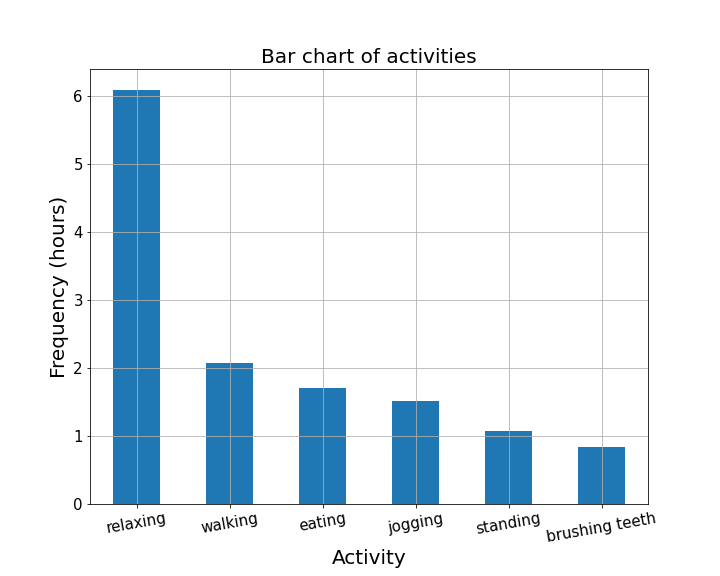
\includegraphics[width=0.85\textwidth, height=0.45\textheight]{Bar_chart_of_activities.png}
	
	\caption{Ραβδόγραμμα κατηγοριών.}
	\label{fig:Bar chart of data}
\end{figure}


{\bf Τα αποτελέσματα της μεθόδου με την διαδικασία αξιολόγησης του \en group 7-Fold cross validation \gr είναι  $accuracy = 0.80$ και $F1 = 0.70$.} Στο σχήμα \ref{fig:Confusion_matrix} παρουσιάζεται ο πίνακας σύγχυσης (\en Confusion matrix) \gr του έβδομου χρήστη, όταν το μοντέλο εκπαιδεύεται στα δεδομένα των πρώτων έξι χρηστών και αξιολογούμε στον έβδομο. Στον κάθετο άξονα βρίσκονται οι πραγματικές κατηγορίες των δεδομένων ενώ στον οριζόντιο οι κατηγορίες που πρόεβλεψε το μοντέλο. Παρατηρούμε ότι τα σφάλματα που γίνονται από το μοντέλο μηχανικής μάθησης έχουν νόημα και δεν είναι αυθαίρετα. Για παράδειγμα, όπως φαίνεται και στο σχήμα \ref{fig:Confusion_matrix}, όταν ο χρήστης καταναλώνει το γεύμα του, πιθανότατα να βρίσκεται και σε κατάσταση ηρεμίας - αδράνειας κίνησης. Έτσι το τελικό μοντέλο προέβλεψε $71\%$ των δεδομένων σώστα ότι ο χρήστης πραγματοποιεί την ενέργεια \en eating \gr και $28\%$ λανθασμένα ότι ο χρήστης πραγματοποιεί την ενέργεια \en relaxing\gr.

Στον πίνακα \ref{tab:10-Fold-Cross-Validation} παραθέτονται {\bf τα αποτελέσματα της μεθόδου μεθόδου με την διαδικασία αξιολόγησης του \en 10-Fold cross validation \gr για κάθε χρήστη ξεχωριστά.} Όπως ήταν αναμενόμενο όταν εκπαιδεύουμε μόνο για τα δεδομένα ενός χρήστη με σκοπό να μπορούμε να καταγράψουμε την μελλοντική συμπεριφορά του, τα αποτελέσματα της μεθόδου είναι εμφανώς καλύτερα. Αυτό μοιάζει λογικό καθώς μαθαίνουμε μόνο για τον συγκεκριμένο χρήστη πως ενεργεί/κινείται σε κάθε δυνατή κατηγορία.

\begin{figure}[H]
	\centering
	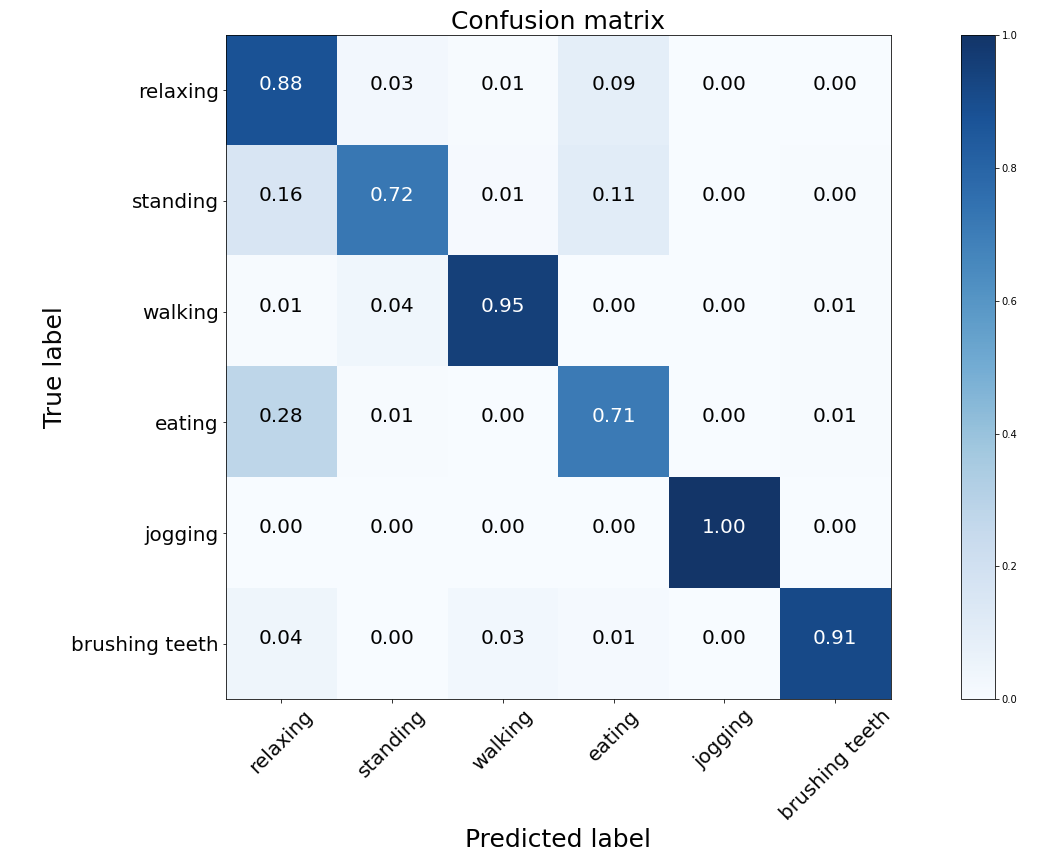
\includegraphics[width=1\textwidth, height=0.5\textheight]{Confusion_matrix_1.png}
	
	\caption{Πίνακας σύγχυσης (\en Confusion matrix\gr).}
	\label{fig:Confusion_matrix}
\end{figure}


\begin{table}[h]
	\centering
	\begin{tabular}{ | c || c || c |}
		\hline
		\en User Id & \en Accuracy & \en F1 \\ 
		\hline
		
		\hline
		0 & 0.99 & 0.98 \\
		
		\hline
		1 & 0.94 & 0.91 \\
		
		\hline
		2 & 0.93 & 0.91 \\
		
		\hline
		3 & 0.91 & 0.84 \\
		
		\hline
		4 & 0.85 & 0.82 \\
		
		\hline
		5 & 0.99 & 0.98 \\
		
		\hline
		6 & 0.95 & 0.95\\
		\hline
		
	\end{tabular}
	\caption{Αποτελέσματα \en 10-Fold cross validation \gr κάθε χρήστη.}
	\label{tab:10-Fold-Cross-Validation}
\end{table}




\section{Βιβλιοθήκες που χρησιμοποιήθηκαν}
Ο κώδικας γράφηκε σε γλώσσα προγραμματιμού \en Python 3\gr  \cite{10.5555/1593511}. Ακολουθούν οι βιβλιοθήκες που χρησιμοποιήθηκαν για την υλοποίηση του προγράμματος.
\begin{itemize}
	\item Για τους μαθηματικούς υπολογισμούς και τον χειρισμό πινάκων χρησιμοποιήθηκε η βιβλιοθήκη \en \href{https://numpy.org/}{numpy} \gr  \cite{harris2020array}.
	
	\item Για τους επιστημονικούς υπολογισμούς χρησιμοποιήθηκε η βιβλιοθήκη \en \href{https://scipy.org/}{scipy} \gr \cite{2020SciPy-NMeth}.
	
	\item Για την επεξεργασία των δεδομένων μέσο \en dataframes \gr χρησιμοποιήθηκε η βιβλιοθήκη \en \href{https://pandas.pydata.org/}{pandas} \gr \cite{reback2020pandas}.
	
	\item Για τα μοντέλα μηχανικής μάθησης έγινε χρήση της βιβλιοθήκης \en \href{https://scikit-learn.org/stable/}{sklearn} \gr \cite{scikit-learn}.
	
	\item H βιβλιοθήκη \en \href{https://matplotlib.org/}{matplotlib} \gr \cite{Hunter:2007} χρησιμοποιήθηκε για τα γραφήματα.
	
\end{itemize}

%\addstarredchapterc{\bibname} % minitoc
\en
\bibliographystyle{ieeetr}
\bibliography{Bibliography}

\end{document}